\textbf{1. Input data.} The physical parameters specified for the closed-closed acoustic tube are
\[
\boxed{L=0.85\,\mathrm{m},\qquad c=340\,\mathrm{m/s},\qquad \rho=1.2\,\mathrm{kg/m}^3,\qquad N=5}\qquad\text{(B.4.1)}
\]
The associated medium properties are the acoustic bulk modulus and the characteristic acoustic impedance:
\[
K=\rho c^2=1.2\times(340)^2\,\mathrm{Pa}=138.72\,\mathrm{kPa},
\qquad
Z=\rho c=1.2\times 340\,\mathrm{Pa\cdot s/m}=408\,\mathrm{rayl}.
\]

\textbf{2. Modal vibration characteristics.} Using the analytical relations derived in Problem B.3, the modal characteristics for modes $j=1,2,3,4,5$ are evaluated as follows:
\par\smallskip\noindent
\textbf{(a) Eigenvalues $z_j$:}
\[
\boxed{z_j=j\pi\quad\Longrightarrow\quad z_1=\pi,\; z_2=2\pi,\; z_3=3\pi,\; z_4=4\pi,\; z_5=5\pi}\qquad\text{(B.4.2.a)}
\]
\textbf{(b) Wavenumbers $\gamma_j$:}
\[
\boxed{\gamma_j=\frac{z_j}{L}=\frac{j\pi}{0.85}\,\mathrm{rad/m}\approx 3.6960\,j\,\mathrm{rad/m}}\qquad\text{(B.4.2.b)}
\]
\textbf{(c) Natural circular frequencies $\omega_j$:} Since $c/L=340/0.85=400\,\mathrm{s}^{-1}$,
\[
\boxed{\omega_j=\gamma_j c=\frac{j\pi c}{L}=400\pi j\,\mathrm{rad/s}\approx 1256.64\,j\,\mathrm{rad/s}}\qquad\text{(B.4.2.c)}
\]
\textbf{(d) Natural frequencies $f_j$ in Hz:}
\[
\boxed{f_j=\frac{\omega_j}{2\pi}=\frac{jc}{2L}=200\,j\,\mathrm{Hz}\quad\Longrightarrow\quad 200,\,400,\,600,\,800,\,1000\,\mathrm{Hz}}\qquad\text{(B.4.2.d)}
\]
The corresponding acoustic wavelengths are $\lambda_j=2L/j=1.70/j\,\mathrm{m}$. The complete modal characteristics are summarized in Table~\ref{tab:hw02-b4-modal}.

\begin{table}[H]
\centering
\caption{Modal vibration characteristics of the closed-closed air tube ($L=0.85\,\mathrm{m}$, $c=340\,\mathrm{m/s}$).}
\label{tab:hw02-b4-modal}
\smallskip
\small
\begin{tabular}{@{}cccccc@{}}
\toprule
Mode $j$ & $z_j$ (rad) & $\gamma_j$ (rad/m) & $\omega_j$ (rad/s) & $f_j$ (Hz) & $\lambda_j$ (m) \\
\midrule
1 & $\pi\approx 3.1416$ & $3.6960$ & $400\pi\approx 1256.64$ & $200$ & $1.7000$ \\
2 & $2\pi\approx 6.2832$ & $7.3920$ & $800\pi\approx 2513.27$ & $400$ & $0.8500$ \\
3 & $3\pi\approx 9.4248$ & $11.0880$ & $1200\pi\approx 3769.91$ & $600$ & $0.5667$ \\
4 & $4\pi\approx 12.5664$ & $14.7840$ & $1600\pi\approx 5026.55$ & $800$ & $0.4250$ \\
5 & $5\pi\approx 15.7080$ & $18.4800$ & $2000\pi\approx 6283.19$ & $1000$ & $0.3400$ \\
\bottomrule
\end{tabular}
\end{table}

\textbf{3. Displacement modeshapes.} From Problem B.3 (item 20), the displacement modeshapes are
\[
\boxed{U_j(x)=\sin\left(\frac{j\pi x}{L}\right)=\sin\left(\frac{j\pi x}{0.85}\right),\qquad j=1,\ldots,5}\qquad\text{(B.4.3)}
\]
Figure~\ref{fig:hw02-b4-disp} plots the displacement modeshapes for the first five modes across the tube length.

\begin{figure}[H]
\centering
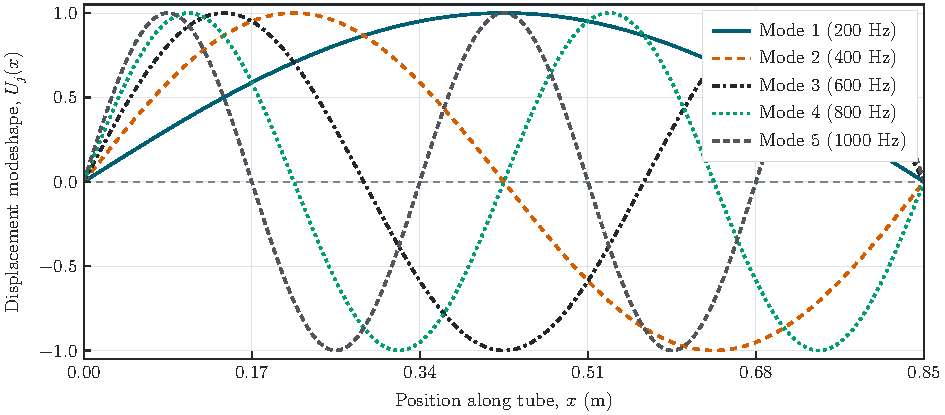
\includegraphics[width=0.96\linewidth]{figures/generated/solutions/B4-displacement.pdf}
\caption{Displacement modeshapes $U_j(x)=\sin(j\pi x/L)$ for modes $j=1,\ldots,5$ in an air tube of length $L=0.85\,\mathrm{m}$ closed at both ends. Ticks along the horizontal axis mark the mode-5 nodal intervals ($x=jL/5$).}
\label{fig:hw02-b4-disp}
\end{figure}

\textbf{4. Discussion of results.}
\begin{itemize}
\item \textbf{Boundary condition verification:} Every displacement modeshape satisfies $U_j(0)=0$ and $U_j(L)=0$ identically. The rigid, impenetrable tube caps at $x=0$ and $x=0.85\,\mathrm{m}$ prevent fluid motion normal to the wall, establishing permanent displacement nodes at both ends.
\item \textbf{Harmonic integer spectrum:} The fundamental resonant frequency is $f_1=200\,\mathrm{Hz}$. Because the eigenvalue spectrum satisfies $z_j=j\pi$, the higher resonance frequencies are exact integer multiples of the fundamental: $f_j=j f_1=200, 400, 600, 800, 1000\,\mathrm{Hz}$. Consequently, a closed-closed tube supports all integer harmonics (both even and odd).
\item \textbf{Wavelength accommodation:} The tube length $L=0.85\,\mathrm{m}$ accommodates an integral number of half-wavelengths for each mode: $L=j(\lambda_j/2)$. For the fundamental mode ($j=1$), only one half of a wave spans the entire tube ($\lambda_1=1.70\,\mathrm{m}=2L$). Each subsequent mode adds another half-wave within the same cavity length.
\item \textbf{Nodes and antinodes:} Mode $j$ contains exactly $j+1$ displacement nodes (including the two ends) and $j$ displacement antinodes where particle amplitude peaks at $|U_j|=1$. The node-to-node spacing is precisely $\Delta x_{\mathrm{node}}=\lambda_j/2=L/j$.
\end{itemize}

\textbf{5. Graduate work: Normalized pressure modeshapes and comparison.}
From Problem B.3 (item 21), acoustic pressure disturbance is generated by fluid strain, $p(x,t)=-Ku_x(x,t)=-\rho c^2 u_x(x,t)$. For displacement amplitude $a_j>0$ in meters, write $u_j(x,t)=a_jU_j(x)e^{-i\omega_jt}$. Differentiating $U_j(x)=\sin(\gamma_jx)$ gives $U_j'(x)=\gamma_j\cos(\gamma_j x)$, yielding the pressure amplitude
\[
P_j(x)=-\rho c^2a_j\gamma_j\cos\left(\frac{j\pi x}{L}\right)=-\rho c\,\omega_j a_j\cos\left(\frac{j\pi x}{L}\right).
\]
\noindent\begin{minipage}{\linewidth}\color{black}
Normalizing by the peak pressure amplitude $|P_j|_{\max}=\rho c\,\omega_j a_j$ yields the normalized pressure modeshape
\[
\boxed{\bar{P}_j(x)=-\cos\left(\frac{j\pi x}{L}\right)=-\cos\left(\frac{j\pi x}{0.85}\right),\qquad j=1,\ldots,5}\qquad\text{(B.4.5)}
\]
\end{minipage}\par

Figure~\ref{fig:hw02-b4-press} plots the normalized pressure modeshapes for modes $1$ through $5$.

\begin{figure}[H]
\centering
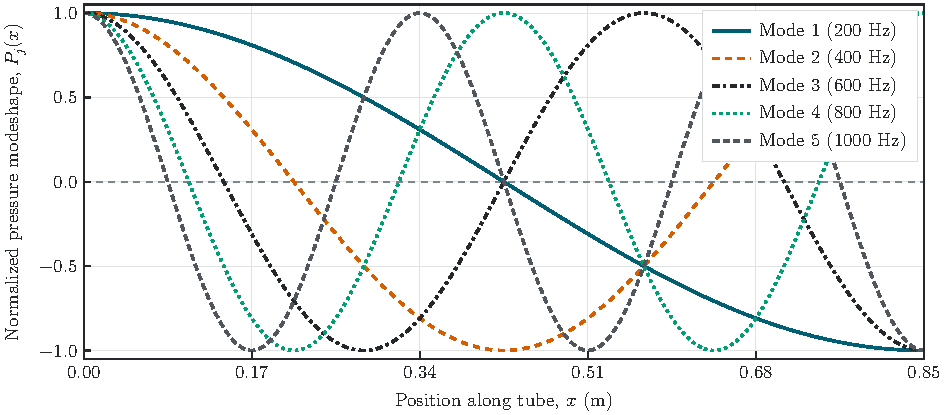
\includegraphics[width=0.96\linewidth]{figures/generated/solutions/B4-pressure.pdf}
\caption{Normalized acoustic pressure modeshapes $\bar{P}_j(x)=-\cos(j\pi x/L)$ for modes $j=1,\ldots,5$ in a closed-closed tube of length $L=0.85\,\mathrm{m}$.}
\label{fig:hw02-b4-press}
\end{figure}

\par\smallskip\noindent
\textbf{Comparison between displacement and pressure modeshapes:}
\par\smallskip\noindent
\textbf{(1) Spatial quadrature ($\pi/2$ phase shift):} Spatial differentiation transforms $\sin(kx)$ into $k\cos(kx)$, introducing a spatial quarter-wavelength ($\pi/2$ radian) shift between displacement and pressure distributions.
\par\smallskip\noindent
\textbf{(2) Boundary behavior:} At the closed caps ($x=0$ and $x=L$), displacement is strictly zero ($U_j=0$, displacement nodes). The displacement gradient has maximum magnitude at these locations, so $p=-Ku_x$ gives maximum pressure magnitude. Consequently, the walls are always pressure antinodes ($|\bar{P}_j(0)|=1$ and $|\bar{P}_j(L)|=1$).
\par\smallskip\noindent
\textbf{(3) Duality of nodes and antinodes:} Wherever particle displacement achieves an antinode ($|U_j|=1$), the spatial gradient is zero ($U_j'=0$), meaning fluid volume change vanishes locally; thus, acoustic pressure disturbance is zero ($\bar{P}_j=0$, pressure nodes). Conversely, at displacement nodes ($U_j=0$), the spatial slope is steepest, creating maximal volumetric strain and therefore pressure antinodes ($|\bar{P}_j|=1$).
\par\smallskip\noindent
\textbf{(4) Nodal counts:} For mode $j$, there are $j$ internal pressure nodes (locations where the acoustic pressure perturbation is zero) and $j+1$ pressure antinodes (including both rigid ends).

\clearpage
\matlabcaption{MATLAB script used to compute modal vibration characteristics and plot displacement and pressure modeshapes for Problem B.4.}

\lstinputlisting[style=hwmatlab]{matlab/B4.m}
